\documentclass{article}

\usepackage{arxiv}
\usepackage[ruled,vlined]{algorithm2e}
\usepackage[utf8]{inputenc}
\usepackage[T1]{fontenc}
\usepackage{url}
\usepackage{booktabs}
\usepackage{amsfonts}
\usepackage{nicefrac}
\usepackage{microtype}
\usepackage{graphicx}
\usepackage[font=small,labelfont=bf]{caption}
\usepackage{cite}
\usepackage{pdflscape}
\usepackage{listings}
\usepackage{outlines}
\usepackage{tikz}

\newcommand*\circled[1]{\tikz[baseline=(char.base)]{
		\node[shape=circle,draw,inner sep=1pt] (char) {#1};}}

\title{Notes on replication in Apache Kafka}

\begin{document}

\section{Log truncation}

Replication in Kafka has evolved from high-watermark- to log-end-offset-based truncation \cite{KIP101} and improved to now prevent replicas from diverging under both clean and unclean leader election \cite{KIP279}.

The current log truncation algorithm relies on the sequence of vectors of \textit{leader epoch} \footnote{also referred to as \textit{generation} in this document} to start offset to ensure replicas are constructed along the same lineage.

When a replica starts to follow a leader, the head of its local log is truncated so that remains only the longest common log prefix of both replicas. In order to do so, the replication algorithm resolves the \textit{fetch offset} the follower must use to truncate to and start replicating from. It searches the latest generation common to both replicas and truncate to the minimum of their respective end offsets. This algorithm is \textit{collaborative} because both leader and follower contribute to the search.

Figure \ref{fig:offsets-for-leader-epoch} exhibits the different steps taken by the algorithm after a sequence of fast broker failovers. In this scenario, two replicas of a topic-partition are considered and unclean leader election is enabled.

\begin{outline}[enumerate]
	\1 Replica 0 is initially the leader and one record is appended to its local log.
	\1 Replica 0 goes offline. Replica 1 is back online and is allowed to acquire leadership because unclean leader election is enabled. One record is appended to the replica.
	\1 Broker 1 is bounced. Note that generation is incremented twice, when broker 1 leaves and rejoins the cluster.
	\1 Three back-to-back unclean leader elections happen with leadership alternating between brokers 0 and 1.
	\1 Replica 0 initiates replication from the leader replica. It first enters the truncation state. Broker 0 sends a \texttt{OffsetsForLeaderEpoch} with the latest generation on the follower, 7. The leader searches for that generation in its local epoch cache. Since it was not online at generation 7, that epoch is not found and the leader returns the largest epoch smaller than 7 it is aware of (5) along with its end offset, defined as the start offset of the generation directly following.
	\1 The follower tries to find the epoch 5 in its local epoch cache, but, since it was offline at that generation, uses the largest preceding generation (1). The end offset for that epoch is the start offset of the directly succeeding epoch (1).
	\1 The follower sends another \texttt{OffsetsForLeaderEpoch} request to inquire about the end offset registered in the leader for epoch 1. The leader is not aware of that epoch, and in that case, does not contain any epoch smaller than it. By design, it returns the same epoch along with the start offset of the first epoch registered in its local sequence.
	\1 The follower observes an epoch from the leader which matches the one requested. It therefore terminates the search and bases its fetch offset off of that epoch, using the minimum end offset between the leader and follower for that epoch.
\end{outline}

Figure \ref{fig:leader-epoch-cache} illustrates the iterative process used to resolve the fetch offset in this example, and shows how the leader and follower collaborates. The offset for epoch 7 is first requested \circled{1}, the vector $(5,2)$ is returned by the leader \circled{2}, leading the follower to resolve the vector $(1,1)$ \circled{3}, then requesting the end offset for that epoch from the leader which responds with vector $(1,0)$ \circled{4}, eventually converging to the fetch offset 0 \circled{5}.



\begin{figure}[h!]
	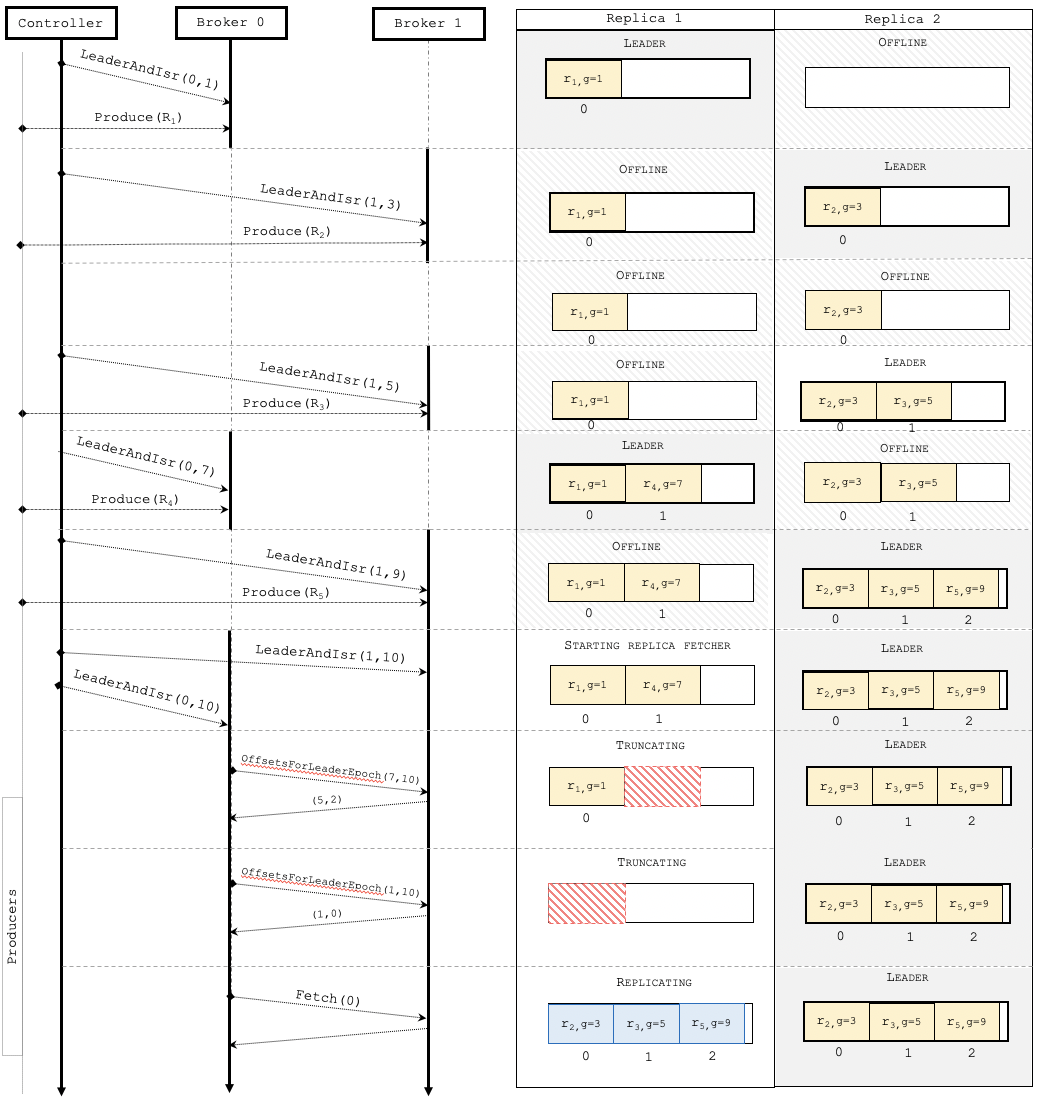
\includegraphics[scale=0.53]{img/offsets-for-leader-epoch.png}
	\captionof{figure}{Back-to-back unclean leader elections resulting in transiently diverging replicas, eventually reconverging through log truncation.}
	\label{fig:offsets-for-leader-epoch}
\end{figure}

\begin{figure}[h!]
	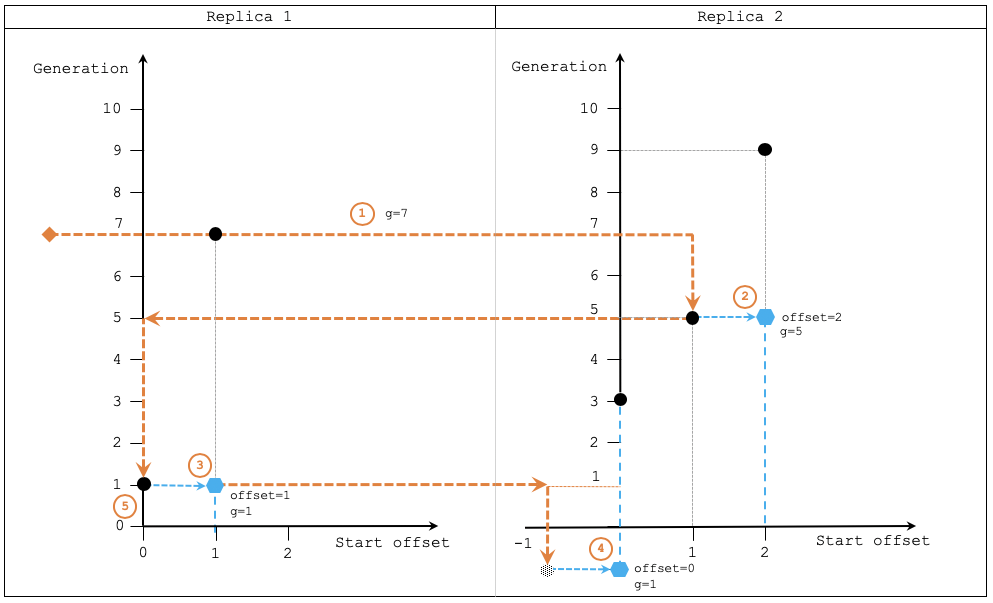
\includegraphics[scale=0.53]{img/leader-epoch-cache.png}
	\captionof{figure}{Round-trips between a leader and follower during the collaborative resolution of the offset to truncate the follower replica to.}
	\label{fig:leader-epoch-cache}
\end{figure}

\bibliography{kafka-replication}{}
\bibliographystyle{plain}
\end{document}


